\section{Basics}

\begin{frame}
\frametitle{An introduction to control}
\end{frame}

\begin{frame}
\frametitle{What is control?}
\begin{itemize}
	\item The goal is to find an input (control signal U(s)) such that the process produces the desired output
	\item Open loop control system: the actual output signal has no effect on the control action
\begin{figure}
\centering
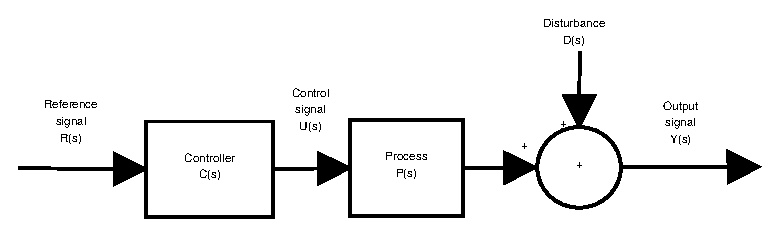
\includegraphics[width=0.7\linewidth]{Open-Loop}
\label{fig:Open-Loop}
\end{figure}
\begin{align*}
	Y = PU = PCR \\
\end{align*}
Remember the example of pouring a glass of water without looking at the glass
\end{itemize}
\end{frame}

\begin{frame}
	\frametitle{A general set-up of a closed loop system}
	\begin{itemize}
		\item We will focus on \underline{closed loop control systems}
		\begin{figure}
\centering
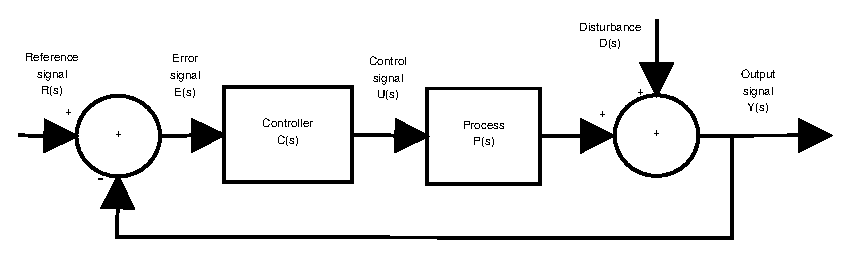
\includegraphics[width=0.7\linewidth]{Closed-Loop}
\label{fig:Closed-Loop}
\end{figure}
\item Example: \href{http://homes.esat.kuleuven.be/~magudelo/_html5/test11.html}{Inverted pendulum}
	\end{itemize}
\end{frame}

\begin{frame}
	\begin{figure}
\centering
\includegraphics[width=0.7\linewidth]{"Inverted Pendulum"}
\caption{Inverted Pendulum}
\label{fig:InvertedPendulum}
\end{figure}
\end{frame}


\begin{frame}
	\frametitle{Concrete Control}
	\begin{itemize}
		\item On-off controller
		\begin{itemize}
			\item Thermostate at home
		\end{itemize}
		\item \textbf{PID controllers, Lead and lag compensators (this course)}
		\begin{itemize}
			\item Cruise-control in your car
		\end{itemize}
		\item More advanced controllers
		\begin{itemize}
			\item STATE-space feedback controllers
			\item Model Predictive Controller (MPC)
			\item Fuzzy Control
			\item Neuro-fuzzy Control
			\item ...
		\end{itemize}
	\end{itemize}
\end{frame}


\section{Control Goals}
\begin{frame}
	\frametitle{What is good control?}
	\begin{itemize}
		\item Before we will start to design control systems we will first focus on the question. What is good control?
		\item It depends on the application
		\begin{itemize}
			\item Stability
			\item Disturbance rejection
			\item Reference tracking (speed)
			\item Sensitivity to errors on model
			\item Etc...
		\end{itemize}
	\end{itemize}
\end{frame}

\begin{frame}
	\frametitle{Examples: stability}
\begin{figure}
\centering
\includegraphics[width=0.7\linewidth]{shuttle}
\caption{Space shuttles are like inverted pendulums. How do you make sure they don't flip over.}
\label{fig:shuttle}
\end{figure}
\end{frame}

\begin{frame}
	\frametitle{Examples: Disturbance rejection}
	\begin{itemize}
		\item Your body will try to keep the temperature in your body as constant as possible. No matter what the outside temperature is. Two people will have almost the same body temperature.
	\end{itemize}
	\begin{figure}
\centering
\begin{minipage}{0.45\textwidth}
\includegraphics[width=0.7\linewidth]{marathon-des-sables}
\caption{Flickr.com, \underline{tent86}, Marathon Des Sables 046}
\label{fig:marathon-des-sables}
\end{minipage}
\centering
\begin{minipage}{0.45\textwidth}
\includegraphics[width=0.7\linewidth]{enduring}
\caption{\underline{Jack Zalium,} Enduring, https://creativecommons.org/licenses/by-nd/2.0/}
\label{fig:enduring}
\end{minipage}
\end{figure}

\end{frame}


\begin{frame}
	\frametitle{Examples: Reference tracking}
	\begin{figure}
\centering
\includegraphics[width=0.7\linewidth]{audi-tracking}
\caption{Audi has a system for automatic driving in traffic jams. The audi will follow the car in front of him at an appropriate distance. \href{https://www.youtube.com/watch?v=Qa_ZSRj0WM0}{youtube}}
\label{fig:audi-tracking}
\end{figure}
\end{frame}

\begin{frame}
	\frametitle{Exercise: name the correct property}
	\begin{figure}
\centering
\includegraphics[width=0.7\linewidth]{ted-drone}
\label{fig:ted-drone}
\end{figure}

\end{frame}